\documentclass[journal,12pt,onecolumn]{IEEEtran}
\usepackage{cite}
\usepackage{graphicx}
\usepackage{amsmath,amssymb,amsfonts,amsthm}
\usepackage{algorithmic}
\usepackage{graphicx}
\usepackage{textcomp}
\usepackage{xcolor}
\usepackage{txfonts}
\usepackage{listings}
\usepackage{multirow}
\usepackage{enumitem}
\usepackage{listings}
\usepackage{pgf-pie}
\usepackage{mathtools}
\usepackage{gensymb}
\usepackage{comment}
\usepackage[breaklinks=true]{hyperref}
\usepackage{tkz-euclide} 
\usepackage{listings}
\usepackage{gvv}                                        
%\def\inputGnumericTable{}                                 
\usepackage[latin1]{inputenc} 
\usetikzlibrary{arrows.meta, positioning}
\usepackage{xparse}
\usepackage{color}                                            
\usepackage{array}                                            
\usepackage{longtable}                                       
\usepackage{calc}                                             
\usepackage{multirow}
\usepackage{multicol}
\usepackage{caption}
\usepackage{hhline}                                           
\usepackage{ifthen}                                           
\usepackage{lscape}
\usepackage{tabularx}
\usepackage{array}
\usepackage{float}
\newtheorem{theorem}{Theorem}[section]
\newtheorem{problem}{Problem}
\newtheorem{proposition}{Proposition}[section]
\newtheorem{lemma}{Lemma}[section]
\newtheorem{corollary}[theorem]{Corollary}
\newtheorem{example}{Example}[section]
\newtheorem{definition}[problem]{Definition}
\newcommand{\BEQA}{\begin{eqnarray}}
\newcommand{\EEQA}{\end{eqnarray}}
\usepackage{float}
%\newcommand{\define}{\stackrel{\triangle}{=}}
\theoremstyle{remark}
\usepackage{circuitikz}
\usepackage{tikz}
\usepackage{wrapfig}
\graphicspath{{figs/}}                                                                       
\title{Graduate Aptitude Test in Engineering 2021}

\author{EE25BTECH11023-Venkata Sai}
\begin{document}
\maketitle
\begin{enumerate}
\item The current population of a city is 11,02,500. If it has been increasing at the rate of 5\% per annum, what was its population 2 years ago?

\begin{multicols}{4}
\begin{enumerate}
\item 9,92,500
\item 9,95,006
\item 10,00,000
\item 12,51,506
\end{enumerate}
\end{multicols}
\hfill (GATE PI 2021)

\item $p$ and $q$ are positive integers and $\frac{p}{q} + \frac{q}{p} = 3,$\
then, $\frac{p^2}{q^2} + \frac{q^2}{p^2} =$

\begin{multicols}{4}
\begin{enumerate}
\item 3
\item 7
\item 9
\item 11
\end{enumerate}
\end{multicols}
\hfill (GATE PI 2021)

\item
The least number of squares that must be added so that the line P-Q becomes the line of symmetry is 

\begin{figure}[H]
    \centering
    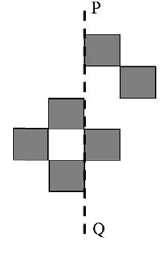
\includegraphics[width=0.3\columnwidth]{figs/fig1.png}
    \caption{}
    \label{fig:placeholder}
\end{figure} 

\begin{multicols}{4}
\begin{enumerate}
\item 4
\item 3
\item 6
\item 7
\end{enumerate}
\end{multicols}
\hfill (GATE PI 2021)

\item \textit{Nostalgia} is to \textit{anticipation} as \dots is to \dots

Which one of the following options maintains a similar logical relation in the above sentence?
\begin{multicols}{4}
\begin{enumerate}
\item Present, past
\item Future, past
\item Past, future
\item Future, present
\end{enumerate}
\end{multicols}
\hfill (GATE PI 2021)

\item Consider the following sentences:\\
(i)  I woke up from sleep.\\
(ii)  I woked up from sleep.\\
(iii) I was woken up from sleep.\\
(iv) I was wokened up from sleep.\\
Which of the above sentences are grammatically CORRECT?
\begin{multicols}{4}
\begin{enumerate}
\item (i) and (ii)
\item (i) and (iii)
\item (ii) and (iii)
\item (i) and (iv)
\end{enumerate}
\end{multicols}

\hfill (GATE PI 2021)


\item
Given below are two statements and two conclusions.\\
Statement 1: All purple are green.\\
Statement 2: All black are green.\\
Conclusion I: Some black are purple.\\
Conclusion II: No black is purple.\\
Based on the above statements and conclusions, which one of the following options is logically CORRECT?
\begin{multicols}{2}
\begin{enumerate}
\item Only conclusion I is correct.
\item Only conclusion II is correct.
\item Either conclusion I or II is correct.
\item Both conclusion I and II are correct.
\end{enumerate}
\end{multicols}
\hfill (GATE PI 2021)

\item
Computers are ubiquitous. They are used to improve efficiency in almost all fields from agriculture to space exploration. Artificial intelligence (AI) is currently a hot topic. AI enables computers to learn, given enough training data. For humans, sitting in front of a computer for long hours can lead to health issues.\\

Which of the following can be deduced from the above passage?\\
(i) Nowadays, computers are present in almost all places.\\
(ii) Computers cannot be used for solving problems in engineering.\\
(iii) For humans, there are both positive and negative effects of using computers.\\
(iv)Artificial intelligence can be done without data.
\begin{multicols}{4}
\begin{enumerate}
\item (ii) and (iii)
\item (ii) and (iv)
\item (i), (iii) and (iv)
\item (i) and (iii)
\end{enumerate}
\end{multicols}
\hfill (GATE PI 2021)

\item
Consider a square sheet of side 1 unit. In the first step, it is cut along the main diagonal to get two triangles. In the next step, one of the cut triangles is revolved about its short edge to form a solid cone. The volume of the resulting cone, in cubic units, is \dots
\begin{multicols}{4}
\begin{enumerate}
\item $\frac{\pi}{3}$
\item $\frac{2\pi}{3}$
\item $\frac{3\pi}{2}$
\item $3\pi$
\end{enumerate}
\end{multicols}
\hfill (GATE PI 2021)


 \item The number of minutes spent by two students, \textbf{X} and \textbf{Y}, exercising every day in a given week are shown in the bar chart above.\

The number of days in the given week in which one of the students spent a minimum of 10\% more than the other student, on a given day, is

\begin{figure}[H]
    \centering
    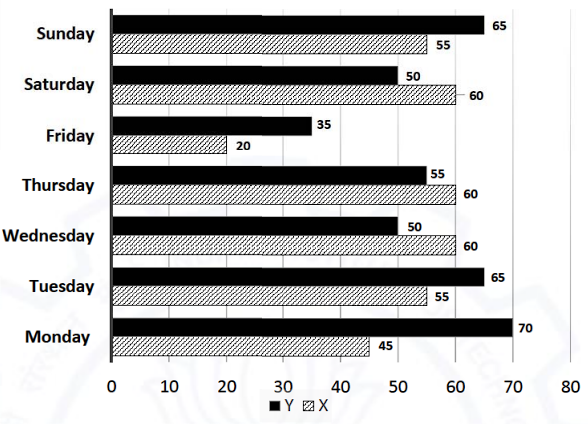
\includegraphics[width=0.5\columnwidth]{figs/fig2.png}
    \caption{}
    \label{fig:placeholder}
\end{figure} 


\begin{multicols}{4}
\begin{enumerate}
\item 4
\item 5
\item 6
\item 7
\end{enumerate}
\end{multicols}

\hfill (GATE PI 2021)

\item
Corners are cut from an equilateral triangle to produce a regular convex hexagon as shown in the figure above.

The ratio of the area of the regular convex hexagon to the area of the original equilateral triangle is

\begin{figure}[H]
    \centering
    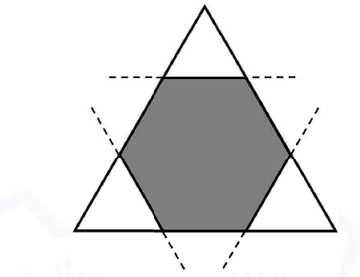
\includegraphics[width=0.5\columnwidth]{figs/fig3.png}
    \caption{}
    \label{fig:placeholder}
\end{figure} 


\begin{multicols}{4}
\begin{enumerate}
\item 2 : 3
\item 3 : 4
\item 4 : 5
\item 5 : 6
\end{enumerate}
\end{multicols}

\hfill (GATE PI 2021)

\end{enumerate}

\newpage
\textbf{Production and Industrial Engineering}
\begin{enumerate}
    
\item
A product has an exponential time-to-failure distribution with a constant failure rate of 0.00006 per hour. The reliability of the product after 4000 hours of operation is

\begin{multicols}{4}
\begin{enumerate}
\item 0.5866
\item 0.6866
\item 0.7866
\item 0.8866
\end{enumerate}
\end{multicols}

\hfill (GATE PI 2021)

\item
In a typical product development process under concurrent engineering approach, all elements of product life cycle from conception to disposal are considered at

\begin{multicols}{2}
\begin{enumerate}
\item Product design stage
\item Process design stage
\item Manufacturing stage
\item Disposal stage
\end{enumerate}
\end{multicols}

\hfill (GATE PI 2021)

\item
When acceptance number of a single sampling plan under attribute category is zero with sample size less than or equal to 10, the Operating Characteristic (OC) curve is

\begin{multicols}{2}
\begin{enumerate}
\item A horizontal line
\item A vertical line
\item A convex function
\item An inverted S-shaped curve
\end{enumerate}
\end{multicols}

\hfill (GATE PI 2021)

\item
Which one of the following is an improvement type heuristic algorithm for computerized layout design technique?

\begin{enumerate}
\item Systematic layout planning (SLP)
\item Computerized relative allocation of facilities technique (CRAFT)
\item Computerized relationship layout planning (CORELAP)
\item Plant layout analysis and evaluation technique (PLANET)
\end{enumerate}

\hfill (GATE PI 2021)

\item
Which one of the following is NOT a measure of forecast error?

\begin{enumerate}
\item Mean absolute deviation (MAD)
\item Mean squared error (MSE)
\item Mean absolute percent error (MAPE)
\item Mean sum product error (MSPE)
\end{enumerate}
\hfill (GATE PI 2021)

\item
llite microstructure in an eutectoid steel consists of alternating layers of two phases, namely $\alpha$ ferrite and
\begin{multicols}{4}
\begin{enumerate}
\item Martensite
\item Austenite
\item Cementite
\item Bainite
\end{enumerate}
\end{multicols}
\hfill (GATE PI 2021)

\item
Which one of the following defects is NOT associated with welding processes?
\begin{multicols}{2}
\begin{enumerate}
\item Angular distortion
\item Hot tear
\item Hydrogen embrittlement
\item Earring
\end{enumerate}
\end{multicols}
\hfill (GATE PI 2021)

\item
Match the component with the corresponding manufacturing process in the table below.\\

\begin{center}
\begin{tabular}{|c|c|c|}
\hline
\textbf{Mineral} & \textbf{Entropy $S^{1,823}$ (kJ K$^{-1}$)} & \textbf{Volume $V^{1,823}$ (J bar$^{-1}$)} \\
\hline
Grossular   & 0.255 & 12.535 \\
\hline
Quartz      & 0.042 & 2.269 \\
\hline
Anorthite   & 0.200 & 10.079 \\
\hline
Wollastonite & 0.082 & 3.993 \\
\hline
\end{tabular}    
\end{center}




\begin{multicols}{4}
\begin{enumerate}
\item P-3, Q-2, R-1, S-4
\item P-3, Q-4, R-2, S-1
\item P-2, Q-3, R-4, S-1
\item P-1, Q-3, R-2, S-4
\end{enumerate}
\end{multicols}

\hfill (GATE PI 2021)

\item
In a turning operation, doubling the cutting speed $\brak{V}$ reduces the tool life $\brak{T}$ to $\brak{\frac{1}{8}}$ of the original tool life. The exponent $n$ in the Taylor's tool life equation, $VT^n = C$ is

\begin{multicols}{4}
\begin{enumerate}
\item $\frac{1}{2}$
\item $\frac{1}{3}$
\item $\frac{1}{4}$
\item $\frac{1}{8}$
\end{enumerate}
\end{multicols}

\hfill (GATE PI 2021)

\item
Which one among the following mechanisms is NOT used for transforming rotation to translation in machine tools?
\begin{multicols}{2}
\begin{enumerate}
\item Screw-nut system
\item 4-bevel gear type differential mechanism
\item Cam and cam follower system
\item Whitworth mechanism
\end{enumerate}
\end{multicols}

\hfill (GATE PI 2021)

\item
Match the measuring feature with the corresponding measuring instrument in the table below.\\

\setlength{\fboxsep}{6pt} % padding inside the box

\begin{center}
\fbox{%
  \begin{minipage}{0.96\textwidth}
    \underline{\textbf{Useful data}}\\[6pt]

    \begin{tabular}{l l}
      Avogadro's Number & : $6.023\times10^{23}\ \mathrm{mol^{-1}}$\\[4pt]
      Boltzmann's constant & : $1.38\times10^{-23}\ \mathrm{J\ K^{-1}}$\\[4pt]
      Electron Charge & : $1.6\times10^{-19}\ \mathrm{C}$\\[4pt]
      Gas Constant & : $8.314\ \mathrm{J\ mol^{-1}\ K^{-1}}$\\[4pt]
      Electron rest mass & : $9.1\times10^{-31}\ \mathrm{kg}$\\[4pt]
      Permittivity of vacuum ($\varepsilon_0$) & : $8.854\times10^{-12}\ \mathrm{F\ m^{-1}}$\\[4pt]
      Planck's constant ($h$) & : $6.62\times10^{-34}\ \mathrm{J\ s^{-1}}$\\[4pt]
      Bohr Magneton ($\mu_B$) & : $9.27\times10^{-24}\ \mathrm{A\ m^{2}}$\\
    \end{tabular}

    \vspace{8pt}

    $1\ \mathrm{eV} = 1.6\times10^{-19}\ \mathrm{J}$\\[2pt]
    $1\ \mathrm{cal} = 4.2\ \mathrm{J}$

    \vspace{10pt}

    \textbf{Atomic weight (in kg mol$^{-1}$) of:}\\[6pt]
    \begin{tabular}{l l}
      Hydrogen & 0.001\\
      Carbon   & 0.012\\
      Nitrogen & 0.014
    \end{tabular}

  \end{minipage}%
}%
\end{center}


\begin{multicols}{4}
\begin{enumerate}
\item P-4, Q-1, R-2, S-3
\item P-1, Q-3, R-4, S-2
\item P-2, Q-4, R-3, S-1
\item P-4, Q-3, R-1, S-2
\end{enumerate}
\end{multicols}

\hfill (GATE PI 2021)

\item
The frequency of pulsing in a die-sinking electric discharge machine (EDM) is 10 kHz. The pulse off-time is set at 40 micro-seconds. The duty factor at this setting is

\begin{multicols}{4}
\begin{enumerate}
\item 0.40
\item 0.60
\item 0.67
\item 2.50
\end{enumerate}
\end{multicols}
\hfill (GATE PI 2021)

\item
A cantilever beam of length 0.3 m is subjected to a uniformly distributed load $C = 10$ kN/m, as shown in the figure. The bending (flexural) rigidity of the beam is 5000 Nm$^2$. Neglecting the self-weight of the beam, the magnitude of beam curvature in m$^{-1}$ at the fixed end is

\begin{figure}[H]
    \centering
    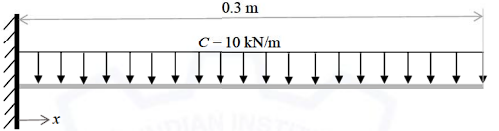
\includegraphics[width=0.5\columnwidth]{figs/fig4.png}
    \caption{}
    \label{fig:placeholder}
\end{figure} 

\begin{multicols}{4}
\begin{enumerate}
\item 1.10
\item 0.02
\item 0.09
\item 0.05
\end{enumerate}
\end{multicols}

\hfill (GATE PI 2021)

\item
A circular rod of length $l = 2$ m is subjected to a compressive load $P$, as shown in the figure. The bending (flexural) rigidity of the rod is 2000 Nm$^2$. If both ends are pinned, then the critical load $P_{cr}$ in N (rounded to the nearest integer) at which the rod buckles elastically is

\begin{figure}[H]
    \centering
    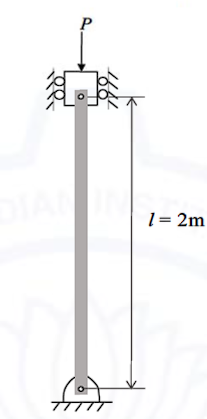
\includegraphics[width=0.3\columnwidth]{figs/fig5.png}
    \caption{}
    \label{fig:placeholder}
\end{figure} 

\begin{multicols}{4}
\begin{enumerate}
\item 4935
\item 2000
\item 5167
\item 1238
\end{enumerate}
\end{multicols}

\hfill (GATE PI 2021)

\item
Two cylindrical parts of equal length $l$, as shown in the figure, made of steel having Young's modulus $E = 200$ GPa and Poisson's ratio $\nu = 0.33$ are press fitted upon one another. If radial interference $\delta = 0.05$ mm, and radii $R = 25$ mm and $R_0 = 40$ mm, then the contact pressure $P$ in MPa at the interface upon press fit is

\begin{figure}[H]
    \centering
    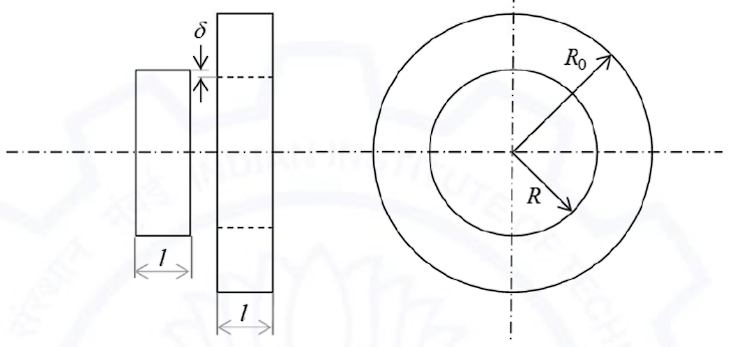
\includegraphics[width=0.5\columnwidth]{figs/fig6.png}
    \caption{}
    \label{fig:placeholder}
\end{figure} 

\begin{multicols}{4}
\begin{enumerate}
\item 10.7
\item 60.9
\item 121.9
\item 1005.3
\end{enumerate}
\end{multicols}

\hfill (GATE PI 2021)

\item
The dimensionless number defined by the ratio of inertial force to viscous force is called
\begin{multicols}{4}
\begin{enumerate}
\item Mach number
\item Froude number
\item Weber number
\item Reynolds number
\end{enumerate}
\end{multicols}
\hfill (GATE PI 2021)

\item
A small capillary tube of 3 mm inner diameter is inserted into a fluid having density 900 kg/m$^3$, surface tension 0.1 N/m, and contact angle $30^\circ$. The rise in the height of fluid in the capillary tube due to surface tension is
\begin{multicols}{4}
\begin{enumerate}
\item 111.4 mm
\item 128.3 mm
\item 89.1 mm
\item 154.1 mm
\end{enumerate}
\end{multicols}

\hfill (GATE PI 2021)

\item
A given steel has identical yield strength of 700 MPa in uni-axial tension and uni-axial compression. If the steel is subjected to pure shear stress such that the three principal stresses are $\sigma_1 = \sigma$, $\sigma_2 = 0$, $\sigma_3 = -\sigma$ with $\sigma_1 \geq \sigma_2 \geq \sigma_3$, then the stress $\sigma$ in MPa for the initiation of plastic yielding in the steel as per von Mises yield criterion is \dots [round off to 2 decimal places]

\hfill (GATE PI 2021)

\item
A cylindrical mild steel tensile test specimen of gauge length 50 mm and diameter 10 mm is extended in two stages at a deformation speed of 4 mm/min. The specimen is extended from 50 mm to 55 mm in the first stage, and from 55 mm to 60 mm in the second stage. Neglecting elastic deformation, the total longitudinal true strain is \dots [round off to 2 decimal places]

\hfill (GATE PI 2021)

\item
A M30 bolt needs to be subjected to pretension $F_i = 350$ kN. If the torque coefficient $K$ of the bolt is 0.2, then the torque in Nm needed to achieve this pretension is \dots [in integer]

\hfill (GATE PI 2021)

\item
A 150 mm wide polyamide flat belt is transmitting 15 kW power through a belt-pulley system. The driving pulley of 150 mm pitch diameter is rotating at 200 RPM. If $F_1$ is the belt tension on high tension side, and $F_2$ is the belt tension on low tension side, then the difference in belt tensions $\Delta F = F_1 - F_2$ in N is \dots [round off to one decimal place]

\hfill (GATE PI 2021)

\item
Heat is being removed from a refrigerator at a rate of 300 kJ/min to maintain its inside temperature at $2^\circ$C. If the input power to the refrigerator is 2 kW, the coefficient of performance of the refrigerator is \dots [round off to one decimal place]

\hfill (GATE PI 2021)

\item
In an ideal Otto cycle, 800 kJ/kg is transferred to air during the constant volume heat addition process and 381 kJ/kg is removed during the constant volume heat rejection process. The thermal efficiency in \% of the cycle is \dots [round off to one decimal place]

\hfill (GATE PI 2021)

\item
If $\brak{3i + 1}x + \brak{4i + 4}y + 5 = 0$ with $x, y$ being real and $i = \sqrt{-1}$, then $x = \dots$ [correct up to one decimal place]

\hfill (GATE PI 2021)

\item
The minimum value of function $f$ defined by\
$f\brak{x, y, z} = x^2 + 5y^2 + 5z^2 - 4x + 40y - 40z + 300$\
is \dots [in integer]

\hfill (GATE PI 2021)

\item
For a given process control chart, there are four rules for determining out-of-control state of the process which are being used simultaneously. The probability of Type-I error for the four rules are 0.005, 0.02, 0.03, and 0.05. Assuming independence of the rules, the probability of overall Type-I error when all the four rules are used simultaneously is

\begin{multicols}{4}
\begin{enumerate}
\item 0.101
\item 0.201
\item 0.001
\item 0.301
\end{enumerate}
\end{multicols}

\hfill (GATE PI 2021)

\item
An in-control process has an estimated standard deviation of 2 mm. The specification limits of the component being processed are 120 $\pm$ 8 mm. When the process mean shifts to 118 mm, the values of the process capability indices, $C_p$ and $C_{pk}$, respectively, are

\begin{multicols}{4}
\begin{enumerate}
\item 1.000, 1.667
\item 1.333, 1.667
\item 1.333, 1.000
\item 1.000, 1.000
\end{enumerate}
\end{multicols}

\hfill (GATE PI 2021)

\item
There are a number of identical components in a parallel system. When the system reliability is 0.97 and the reliability of each individual component is 0.68, the number of identical components in the system is (if actual value is a fraction, it may be rounded up to the next higher integer).

\begin{multicols}{4}
\begin{enumerate}
\item 2
\item 4
\item 6
\item 8
\end{enumerate}
\end{multicols}

\hfill (GATE PI 2021)

\item
A retail chain company has identified four sites A, B, C and D to open a new retail store. The company has selected four factors as the basis for evaluation of these sites. The factors, their weights, and the score for each site are given in the following table.


\begin{center}
\begin{tabular}{|c|c|c|c|}
\hline
   {S.No}  & {Production Alternatives} & {Unit Cost (Rs.)} & {Capacity /month}  \\ \hline
   1  & Regular time production & 5 & 300 \\ \hline
   2 & Overtime production & 6 & 200 \\ \hline
   3 & Subcontracting & 10 & 500 \\ \hline
\end{tabular}
\end{center}

The site that should be selected to open the new retail store is

\begin{multicols}{4}
\begin{enumerate}
\item Site A
\item Site B
\item Site C
\item Site D
\end{enumerate}
\end{multicols}

\hfill (GATE PI 2021)

\item
In the classical economic order quantity (EOQ) model, let $Q$ and $C$ denote the optimal order quantity and the corresponding minimum total annual cost (the sum of the inventory holding and ordering costs). If the order quantity is estimated incorrectly as $Q' = 2Q$, then the corresponding total annual cost $C'$ is

\begin{multicols}{4}
\begin{enumerate}
\item $C' = 1.25C$
\item $C' = 1.5C$
\item $C' = 1.75C$
\item $C' = 2C$
\end{enumerate}
\end{multicols}

\hfill (GATE PI 2021)

\item
The eigenvalues of matrix 
$
\myvec{
8 & 3\\
2 & 7
}
$
are 5 and 10. For matrix $B = A + \alpha I$, where $\alpha$ is a constant and $I$ is $2 \times 2$ identity matrix, its eigenvalues are

\begin{multicols}{4}
\begin{enumerate}
\item 5, 10
\item $5 + \alpha,\ 10 + \alpha$
\item $5 - \alpha,\ 10 - \alpha$
\item $5\alpha,\ 10\alpha$
\end{enumerate}
\end{multicols}

\hfill (GATE PI 2021)

\item
A company manufactures two products P and Q with unit profit of 4 and 5, respectively. The production requires manpower and two kinds of raw materials R1 and R2. The following table summarizes the requirement and availability of resources.


\begin{center}
\begin{tabular}{lcc}
 & {Automat} & {Center Lathe} \\
\hline
Machine Setup Time (min) & 120 & 30 \\ \hline
Machine Setup Cost (Rs./min) & 800 & 150 \\ \hline
Machining Time per piece (min) & 2 & 25 \\ \hline
Machining Cost (Rs./min) & 500 & 100 \\ \hline \\
\end{tabular}
\end{center}
The maximum profit the company can make is

\begin{multicols}{4}
\begin{enumerate}
\item 45
\item 48
\item 42
\item 54
\end{enumerate}
\end{multicols}

\hfill (GATE PI 2021)

\item
A tool of an NC machine has to move along a circular arc from $\brak{20,20}$ to $\brak{10,10}$, while performing an operation. The center of the arc is at $\brak{20,10}$. Which one of the following NC tool commands performs the above mentioned operation?

\begin{enumerate}
\item N020 G03 X20 Y20 X10 Y10 R10
\item N020 G02 X20 Y20 X10 Y10 R10
\item N020 G02 X10 Y10 X20 Y20 R10
\item N020 G01 X20 Y20 X10 Y10 R10
\end{enumerate}

\hfill (GATE PI 2021)

\item
In a shaft-hole assembly, the hole is specified as $30^{0.040}_{0.000}$ mm. The mating shaft has a clearance fit with minimum clearance of 0.01 mm. The tolerance on the shaft is 0.03 mm. The maximum clearance in mm between the hole and the shaft is

\begin{multicols}{4}
\begin{enumerate}
\item 0.04
\item 0.05
\item 0.08
\item 0.10
\end{enumerate}
\end{multicols}

\hfill (GATE PI 2021)

\item
'GO' and 'NO GO' snap gauges are to be designed for a shaft 36.000$^{+0.070}_{+0.010}$ mm. Gauge tolerance can be taken as 5\% of the hole tolerance. Following the ISO system of gauge design, the respective sizes of 'GO' and 'NO GO' gauges are

\begin{multicols}{2}
\begin{enumerate}
\item 36.013 mm and 36.067 mm
\item 36.015 mm and 36.065 mm
\item 36.018 mm and 36.062 mm
\item 36.020 mm and 36.060 mm
\end{enumerate}
\end{multicols}

\hfill (GATE PI 2021)

\item
A circular tank of 4 m diameter is filled up to a height of 3 m. Assuming almost steady flow and neglecting losses, the time taken in seconds to empty the tank through a 5 cm diameter hole located at the center of the tank bottom (take acceleration due to gravity $g = 9.81$ m/s$^2$) is \dots [round off to the nearest integer]

\begin{multicols}{4}
\begin{enumerate}
\item 5005
\item 1807
\item 8097
\item 3154
\end{enumerate}
\end{multicols}

\hfill (GATE PI 2021)

\item
The probability mass function $P\brak{x}$ of a discrete random variable $X$ is given by $P\brak{x} = \frac{1}{2^x}$, where $x = 1, 2, \dots, \infty$. The expected value of $X$ is \dots [in integer]

\hfill (GATE PI 2021)

\item
The time to pass through a security screening at an airport follows an exponential distribution. The mean time to pass through the security screening is 15 minutes. To catch the flight, a passenger must clear the security screening within 15 minutes. The probability that the passenger will miss the flight is \dots [round off to 3 decimal places]

\hfill (GATE PI 2021)

\item
A machine shop has received four jobs A, B, C and D for processing on a single CNC machine. All jobs are available for processing on the first day of the production schedule calendar, and processing times and due dates as applicable on the first day are given below. Using earliest due date rule, the average tardiness (in days) is \dots [in integer]

\begin{table}[H]
    \centering
    \begin{tabular}{c|c}
      GROUP I & GROUP II \\
        P.Polyester & I. Ethylene Glycol\\
        Q. Polyamide & II. Adipic acid\\
        R. Viscous rayon & III. Cellulose\\
        S. Epoxy resin & IV. Bisphenol
    \end{tabular}
    \caption{Table-5}
    \label{tab:tables/table5.tex}
\end{table}


\hfill (GATE PI 2021)

\item
A time study is carried out for a spot welding operation which is being performed by an operator. The time taken (in seconds) for five observations are recorded as 40, 35, 45, 37 and 43, respectively. If the standard time and the allowance for this operation are 45 seconds and 9 seconds, respectively, then the performance rating (in percentage) of the operator is \dots [in integer]

\hfill (GATE PI 2021)

\item
The initial cost of a machine is INR 10,00,000 and its salvage value after 10 years of use is INR 50,000. Using the straight line depreciation method, the book value in INR of the machine at the end of 7$^\mathrm{th}$ year is \dots [in integer]

\hfill (GATE PI 2021)

\item
A project consists of eight activities. The time required for each activity and its immediate predecessor(s) are given in the table below.

\begin{center}
\begin{tabular}{|c|c|c|}
\hline
\textbf{Activity} & \textbf{Activity time (in days)} & \textbf{Immediate predecessor(s)} \\
\hline
A & 2 & - \\
B & 3 & - \\
C & 2 & A \\
D & 4 & A, B \\
E & 4 & C \\
F & 3 & C \\
G & X & D, E \\
H & 2 & F, G \\
\hline
\end{tabular}
\end{center}


If the project completion time using critical path method (CPM) is 15 days, then the value of X (in days) is \dots [in integer]

\hfill (GATE PI 2021)

\item
A wire of 5 mm diameter is drawn into a wire of 4 mm diameter through a conical die at a constant pulling speed of 5 m/s. Neglecting the coefficient of friction and redundant work, the drawing stress $\brak{\sigma_d}$ in MPa for the above process is given by $\sigma_d = \bar{\sigma} \ln \brak{\frac{1}{1-r}}$, where $\bar{\sigma}$ is the mean flow strength of wire material in MPa, and $r$ is the ratio of decrease in area of cross-section to initial area of cross-section of the wire. If the mean flow strength of wire material is 600 MPa, then the power required in kW in the above wire drawing process is \dots [round off to 2 decimal places]

\hfill (GATE PI 2021)

\item
In an arc welding process, the DC power source characteristic is linear with an open circuit voltage of 60 V and short circuit current of 600 A. The heat required for melting a metal during the welding is 10 J/mm$^3$, and the heat transfer and melting efficiencies are 80\% and 25\%, respectively. If the weld cross-sectional area of 20 mm$^2$ is made using the maximum arc power, then the required welding speed in mm/s is \dots [round off to one decimal place]

\hfill (GATE PI 2021)

\item
A company is producing a disc-shaped product of 50 mm thickness and 1.0 m diameter using sand casting process. The solidification time of the above casting process is estimated by Chvorinov's equation $t = B \brak{\frac{V}{A}}^2$, where $B$ is the mold constant, and $V$ and $A$ are the volume and surface area of the casting, respectively. It is decided to modify both the thickness and diameter of the disc to 25 mm and 0.5 m, respectively, maintaining the same casting condition. The percentage reduction in solidification time of the modified disc as compared to that of the bigger disc is \dots [round off to one decimal place]

\hfill (GATE PI 2021)

\item
A single point cutting tool with $15^\circ$ orthogonal rake angle is used to machine a mild steel plate under orthogonal machining condition. The depth of cut (uncut thickness) is set at 0.9 mm. If the chip thickness is 1.8 mm, then the shear angle in degree is \dots [round off to one decimal place]

\hfill (GATE PI 2021)

\item
The top layer of a flat 750 mm $\times$ 300 mm rectangular mild steel plate is to be machined with a single depth of cut using a shaping machine. The plate has been fixed by keeping 750 mm side along the tool travel direction. If the approach and the over-travel are 25 mm each, average cutting speed is 10 m/min, feed rate is 0.4 mm/stroke, and the ratio of return time to cutting time of the tool is 1:2, the time (in minutes) required to complete the machining operation is \dots [round off to one decimal place]

\hfill (GATE PI 2021)

\item
A 3 mm thick steel sheet, kept at room temperature of 30$^\circ$C, is cut by a fiber laser beam. The laser spot diameter on the top surface of the sheet is 0.2 mm. The laser absorptivity of the sheet is 50\%. The properties of steel are density $= 8000$ kg/m$^3$, specific heat $= 500$ J/kg.$^\circ$C, melting temperature $= 1530^\circ$C, and latent heat of fusion $= 3\times10^5$ J/kg. Assume that melting efficiency is 100\% and that the kerf width is equal to the laser spot diameter. The maximum speed (in m/s) at which the sheet can be fully cut at 2 kW laser power is \dots [round off to 3 decimal places]

\hfill (GATE PI 2021)

\item
In a point-to-point open-loop NC drive, a stepper motor with $1.8^\circ$ step angle is coupled to a leadscrew through a gear reduction of 4:1 (4 rotations of the motor enables 1 rotation of leadscrew). The single-start leadscrew has a pitch of 4 mm. The worktable of the system is driven by the leadscrew. If the table moves at a uniform speed of 10 mm/s, the pulse frequency (in Hz) required to drive the stepper motor is \dots [round off to one decimal place]

\begin{figure}[H]
    \centering
    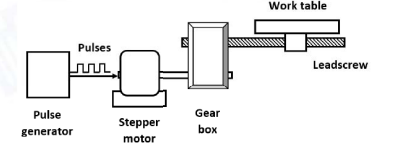
\includegraphics[width=0.5\columnwidth]{figs/fig7.png}
    \caption{}
    \label{fig:placeholder}
\end{figure} 

\hfill (GATE PI 2021)

\item
A 30 kg smooth, solid sphere rests on two frictionless inclines as shown in the figure. The magnitude of contact force in N acting at the point A is (take acceleration due to gravity $g = 9.81$ m/s$^2$ and consider both sphere and inclines to be rigid) \dots [round off to 2 decimal places]

\begin{figure}[H]
    \centering
    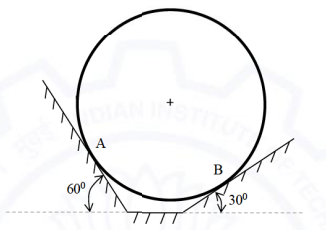
\includegraphics[width=0.5\columnwidth]{figs/fig8.png}
    \caption{}
    \label{fig:placeholder}
\end{figure} 

\hfill (GATE PI 2021)

\item
Consider the truss shown in the figure. The members AB, BC, and CA are all rigid and form an equilateral triangle. The contact between roller and ground at C is frictionless. If the self-weight of members is neglected, the force in member BC in N is (negative sign should be used if the force is compressive and positive if the force in the member is tensile) \dots [round off to one decimal place]

\begin{figure}[H]
    \centering
    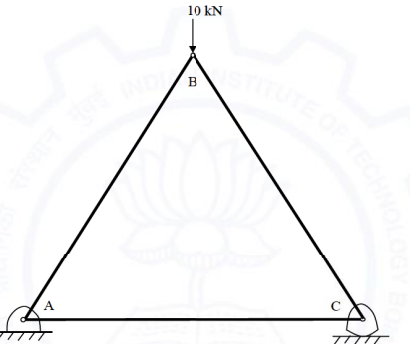
\includegraphics[width=0.5\columnwidth]{figs/fig9.png}
    \caption{}
    \label{fig:placeholder}
\end{figure} 

\hfill (GATE PI 2021)

\item
A fluid with dynamic viscosity $\mu = 1$ Pa.s is flowing through a circular pipe with diameter 1 cm. If the flow rate (discharge) in the pipe is 0.2 liter/s, the maximum velocity in m/s of the fluid in the pipe is (assume fully developed flow and take fluid density $\rho = 1000$ kg/m$^3$) \dots [round off to one decimal place]

\hfill (GATE PI 2021)

\item
Values of function $y\brak{x}$ at discrete values of $x$ for $0 \leq x \leq 10$ are given in table. Using trapezoidal rule, $\int_0^{10} y\brak{x} dx =$ \dots [round off to one decimal place]


\begin{center}
\begin{tabular} {|c|c|c|} 
\hline \\
{Group 1} & {Group 2} \\ \hline
P. Man\--machine chart &  1.Determines standard time of jobs \\ \hline
Q. Learning curve  &  2. Finds the preferred method of doing work \\ \hline 
R. Time study  & 3. Measures work improvement  \\ \hline
S. Motion study  & 4. Shows idle times  \\ \hline
\end{tabular}
\end{center}

\hfill (GATE PI 2021)

\item
Temperature field inside a sphere of radius $R = 1$ m with origin at its center is $T\brak{x,y,z} = 100 - 70x + 51y - 80z - 10x^2 - 20y^2 - 20z^2$. If thermal conductivity of the sphere material is $K = 50$ W/m.K and Fourier law of heat conduction is valid, net heat leaving the sphere per unit time in W is \dots [round off to one decimal place]

\hfill (GATE PI 2021)

\item
A 3.5 mm thick sheet is rolled using a two high rolling mill to reduce the thickness under plane strain condition. Both rolls have a diameter of 500 mm and are rotating at 200 RPM. The coefficient of friction at the sheet and roll interface is 0.08, and the elastic deflection of the rolls is negligible. If the mean flow strength of the sheet material is 400 MPa, then the minimum possible thickness (in mm) of sheet that can be produced in a single pass is \dots [round off to 2 decimal places]

\hfill (GATE PI 2021)
\end{enumerate}

\end{document}